\documentclass{school-22.211-notes}
\date{February 22, 2012}

\begin{document}
\maketitle

%%%%%%%%%%%%%%%%%%%%%%%%% Resonance Day 2: Important Parameters %%%%%%%%%%%%%%%%%%%%%%%%%%%%
\clearpage
\topic{Important Parameters}
\subtopic{Resonance Integrals}
We introduce \hi{(Infinite) Resonance Integrals} as flux weighted (that is, weighted with 1/E spectrum $\phi(E) \sim \frac{1}{E}$) microscopic cross section: 
\begin{align}
\RI &=  - \int_{u1}^{u2} \sigma(u) \du \\
u &= \ln \left( \frac{E_0}{E} \right) = \ln(E_0) - \ln E \\
\du &= - \frac{1}{E} \dE \\ 
\RI &=  \int \sigma (E) \frac{1}{E} \dE 
\end{align}
Notice, 
\begin{itemize}
\item RI is defined directly from cross section data; no flux calculation is required because 1/E spectrum is assumed; 
\item RI depends on the normalization of the 1/E flux spectrum; it is also implicitly assumed that flux equals 1 when $E = 1$ through normalization;
\item RI is independent of energy bounds for isolated resonances;
\item RI is independent of temperature. This is because if the energy bound is larger enough, then as temperature increases, the spectrum would broaden, but because the area under the curve remains the same, assume the cross section is constant, then RI is essentially integrating the spectrum, which would not change upon temperature change;
\item RI is useful for inter-comparing libraries or cross section models. It is a classic way to evaluate new resonance data typically from 0.5 eV to 10 keV. We use RI to check our resonance data, in particularly the three big resonances at 6.67, 20.9, 36.7, 66 eV. Numerical test of the SLBW RIs shows that the RI comes out to be within 1\% of ENDF/B-VII Reich-Moore data (Lec 6, slide 17, with 0.01 eV as spacing in histogram). 
\end{itemize}


\subtopic{Group Cross Section}
Group cross section is a similar but much more useful quantity. From its definition, we see $\sigma_g$ does not depend on the flux normalization: 
\begin{align}
\sigma_g &= \frac{\int_{E_1}^{E_2} \sigma(E) \phi(E) \dE }{\int_{E_1}^{E_2} \phi(E) \dE} 
\end{align}
If we make assumptions on the flux spectrum, then we can relate $\sigma_g$ to $\RI_{\eff}$,
\begin{align}
\phi(E) &\sim \frac{1}{E} \\
\sigma_g &= \frac{\int_{E_1}^{E_2} \sigma(E) \frac{1}{E} \dE }{\int_{E_1}^{E_2} \frac{1}{E} \dE} 
= \frac{\RI_{\eff}}{\ln(E_2) - \ln(E_1)}  
= \frac{\RI_{\eff}}{\ln(E_2/E_1)} \\
\Aboxed{\RI_{\eff} &= \sigma_g \ln(E_2/E_1) } \label{RIeff}
\end{align}
Notice\footnote{Review here for exam}:
\begin{itemize}
\item Group cross section by definition depends on both cross section and flux spectrum. 
\item Group cross section depends on the flux, but not on the normalization of flux (that is, only the shape matters, not the magnitude);
\item Group cross section depend explicitly on energy bounds (widths) of the groups; 
\item Effective RI can be computed from group cross sections and group energy bounds as in Eq.~\ref{RIeff}; As spectrum approaches 1/E, the effective RI computed from group cross sections will approach infinite RI. 
\end{itemize}

\clearpage
\subtopic{Dilution Cross Section/Dilution Factor}
In an infinite homogeneous medium with one resonance absorber and one moderator,  we write removal rates equals scattering rates (see Reuss 8.2.1 for a similar derivation), 
\begin{align}
\left[ N_r \sigma_r (u) + N_m \sigma_m (u) \right] \phi (u) &= \int_{-\infty}^u N_m \sigma_m (u') \phi(u') P(u' \to u) \du' \\ 
&= N_m \sigma_m \int_{-\infty}^u \phi(u') P(u' \to u) \du' \\
&= N_m \sigma_m C \\
\phi(u) &\propto \frac{N_m \sigma_m}{N_r \sigma_r(u) + N_m \sigma_m} \\
\phi(u) &\propto \frac{ \frac{N_m}{N_r} \sigma_m}{\sigma_r(u) + \frac{N_m}{N_r} \sigma_m}  \label{flux-shape}
\end{align}
In the above derivation we made two assumptions:
\begin{itemize}
\item The moderator's xs is independent of energy near resonances. For almost any moderators we can pick, the assumption that the elastic scattering xs is constant is valid in the thermal range as in Figure~\ref{scatter-xs}. 
\item $\int \phi(u') P(u' \to u) \du'$ is constant. We know that the flux above the resonance is 1/E and hence constant in lethargy. If we assume scattering into the resonance comes from this constant lethargy region, then the resonance lethargy is constant as well. 
\end{itemize}
Eq.~\ref{flux-shape} suggests that \textit{in infinite medium the flux shape near resonance depends only on the ratio of the number density of the moderator to the resonance absorber and the moderator cross section.} But once we move into a finite medium or we take into account leakage, then the absolute number densities are needed.
 
To capture the ratio of number densities and the moderator cross section, we define \hi{dilution cross section} as,
\eqn{ \boxed{ \sigma_d = \frac{N_m \sigma_m}{N_r} } }
Then the flux shape near resonance is,
\eqn{ \boxed{ \phi(u) \propto \frac{\sigma_d}{\sigma_r + \sigma_d} } }
This flux shapes let us to compute approximated effective RI. Recall RI is defined as, $\RI = \int \sigma_r (u) \du$. Then the approximated effective RI is,
\eqn{ \boxed{ \RI_{\eff} = \int \sigma_r(u) \frac{\sigma_d}{\sigma_r + \sigma_d} \du }  }
Two extremes of $\RI_{\eff}$ and $\sigma_d$:
\begin{itemize}
\item As $\sigma_d \to \infty$, the entire media is moderator, we reach the limit of infinite dilute, $\RI_{\eff} \to \RI$; we should get within 1\% of the ENDFVII xs data;
\item As $\sigma_d \to 0$, analytically our assumptions do not hold true any more, but the MC is true that as $\RI_{\eff} \to 0, \phi \to 0$ as seen in Figure~\ref{energy-self-shielding}. Interpretation: as we have no moderator, every atom is essentially self-shield because they are all resonant isotopes, hence infinite flux depression.  
\end{itemize}
The scattering down to resonance is independent of the resonance. In other words, if the spectrum above a resonance returns to 1/E as in Figure~\ref{1overE}, the group cross sections will be independent of higher energy absorptions. This may be related to what we talk about before, that 
\begin{figure}
  \centering
  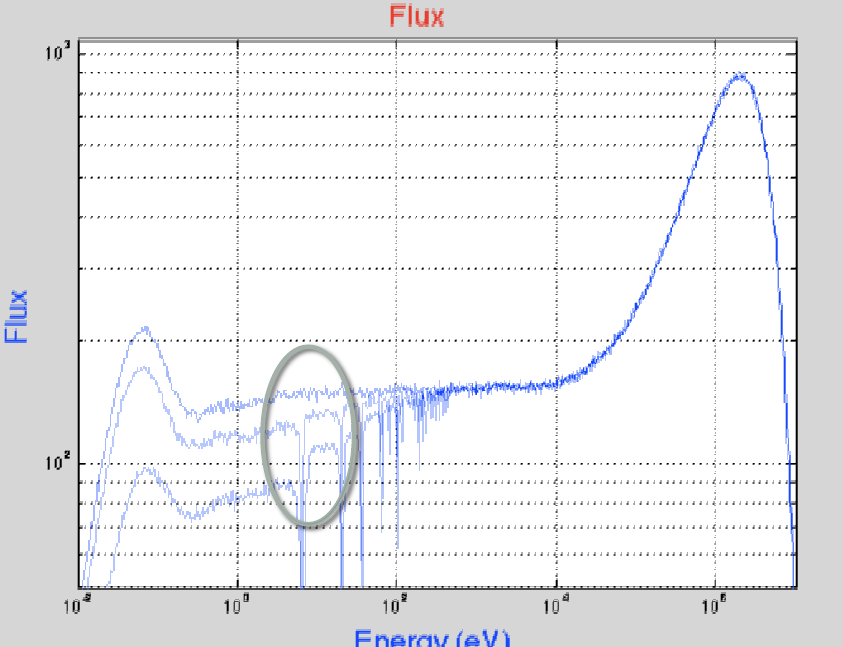
\includegraphics[width=3in]{images/r-m/resonance-1-over-E.png}
  \caption{The 1/E Spectrum Above A Resonance Suggests Group XS Independent of Higher Energy Absorption} \label{1overE}
\end{figure}



%%%%%%%%%%%%%%%%%%%%%%%%% RESONANCE ESCAPE PROBABILITY %%%%%%%%%%%%%%%%%%%%%%%%
\clearpage
\subtopic{Resonance Escape Probability}
We define $p$ as the ratio of the therm neutron absorption rate over absorption rate at all energies; it is the fraction of neutrons absorbed thermally over all neutrons absorbed in the cell; hence it is the probability that a neutron will escape capture at energies above thermal; finally since most of the non-thermal capture in natural or slightly enriched uranium lattices is in the resonance part of the slowing down region, it is the \hi{resonance escape probability}\footnote{Henry, p. 110}. 
\begin{align}
p &= \exp \left( - \frac{N_R \RI_{\eff}}{\xi \Sigma_m} \right)  = \exp \left( - \frac{\RI_{\eff}}{\xi \sigma_d} \right)
\end{align}
Notice: (1) this expression is only an approximation; (2) \textit{p only depends on effective RI and dilution cross section.} For instance, in a hydrogen system with $\sigma_d = 200$, we can tabulate the p values as in Table~\ref{p-values}. The last entry tells us that \textit{about 20\% of neutrons are absorbed in U238 resonances.}
\begin{table}
  \centering
  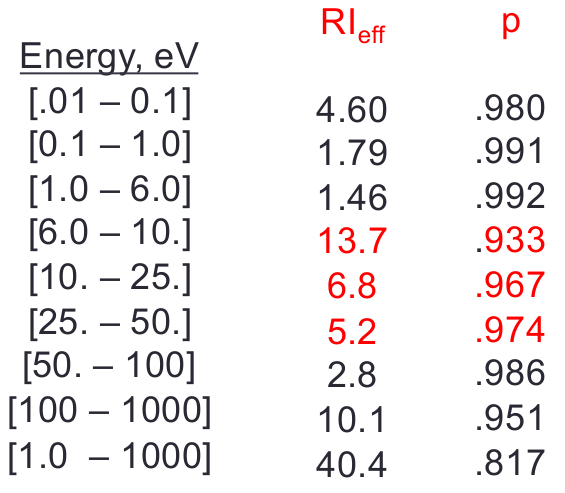
\includegraphics[width=1.5in]{images/r-m/resonance-escape-probability.png}
  \caption{Resonance Escape Probability For A Hydrogen System} \label{p-values}
\end{table}

\textbf{Derivation of $p$ expression:}
\begin{enumerate}
\item Assumptions: only elastic down scatter above the resonance, $\sigma_{a,m} = 0, \sigma_{s} = $const, and only a single resonance absorber. 
\item Start from our balance equation (scattering in = resonance absorption),
\begin{align}
\frac{S}{\zeta(u)} \du &= \left[ N_r \sigma_{a,r} (u) + \Sigma_m \right] \phi(u) \du = N_r \left[ \sigma_{a,r} (u) + \sigma_d \right] \phi(u) \du \\
\Rightarrow \phi(u) &= \frac{S}{\zeta(u) N_r \left[ \sigma_{a,r} (u) + \sigma_d \right] } 
\end{align}
Define resonance escape probability as:
\begin{align}
p &= \frac{S - \int N_r \sigma_a(u) \phi(u) \du}{S} \\
&= 1 - \frac{\int N_r \sigma_a(u) \frac{S}{\zeta(u) N_r \left[ \sigma_{a,r} (u) + \sigma_d \right] } \du }{S} \\
&= 1 - \int \frac{\sigma_{a,r} (u) }{\zeta(u) \left[ \sigma_{a,r} (u) + \sigma_d \right] } \du
\end{align}
\item Assume the mean logarithmic energy decrement is independent of lethargy, 
\eqn{ p = 1 - \frac{1}{\zeta} \int \frac{\sigma_{a,r} (u)}{\sigma_{a,r} (u) + \sigma_d} \du }
\item Use our definition of effective RI,
\eqn{ \RI_{\eff}^{u1 \to u2} = \int_{u1}^{u2} \frac{\sigma_{a,r} (u) \sigma_d}{\sigma_{a,r} (u) + \sigma_d} \du }
We can write $p$ in terms of $\RI$:
\eqn{ \boxed{p^{1\to 2} = 1 - \frac{\RI_{\eff}^{u1 \to u2}}{\zeta \sigma_d} } }
\item Since the source is incrementally reduce with each successive resonance,
\eqn{ p^{u1 \to uN} = \left( 1 - \frac{\RI_{\eff}^{u1 \to u2}}{\zeta \sigma_d} \right) \left( 1 - \frac{\RI_{\eff}^{u2 \to u3}}{\zeta \sigma_d} \right)
  \cdots \left( 1 - \frac{\RI_{\eff}^{uN-1 \to uN}}{\zeta \sigma_d} \right) }
We approximate the sequence as,
\eqn{ p^{u1 \to uN} = \exp \left( - \frac{\Sum_{u1}^{uN-1} \RI_{\eff}^u}{\zeta \sigma_d} \right) }
or
\eqn{ \boxed{ p \approx \exp \left( - \frac{\RI_{\eff}}{\zeta \sigma_d} \right) = \exp \left( - \frac{N_r \RI_{\eff}}{\zeta \Sigma_m} \right)  } }
which for hydrogen system becomes, 
\eqn{ p \approx \exp \left( - \frac{\RI_{\eff}}{\sigma_d} \right) }
\end{enumerate}






\end{document}
